% Author: Izaak Neutelings (February 2020)
% http://texample.net/tikz/examples/tag/circuitikz/
% http://texample.net/tikz/examples/circuitikz/
% https://www.overleaf.com/learn/latex/CircuiTikz_package
% http://texdoc.net/texmf-dist/doc/latex/circuitikz/circuitikzmanual.pdf
% http://repositorios.cpai.unb.br/ctan/graphics/pgf/contrib/circuitikz/circuitikzmanual.pdf
\documentclass[border=3pt,tikz]{standalone}
\usepackage{amsmath} % for \dfrac
\usepackage{physics}
\usepackage{tikz,pgfplots}
\usepackage[siunitx]{circuitikz} %[symbols]
\usepackage{xcolor}
\tikzset{>=latex} % for LaTeX arrow head
\colorlet{Icol}{blue!50!black}
\colorlet{Ccol}{orange!90!black}
\colorlet{pluscol}{red!60!black}
\colorlet{minuscol}{blue!60!black}
%\tikzstyle{charged}=[top color=blue!20,bottom color=blue!40,shading angle=10]
\tikzstyle{thick C}=[C,thick,color=Ccol,Ccol,l=$C$]
\tikzstyle{mybattery}=[battery1,l=$\Delta V$,invert]


\begin{document}


% CAPACITOR without battery
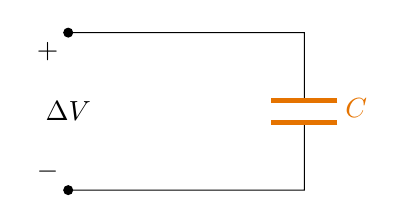
\begin{tikzpicture}
  \draw (0,2) to [short,*-] (3,2) to[thick C] (3,0) to [short,-*] (0,0);
  \node[below left] at (0,2) {$+$};
  \node[above left] at (0,0) {$-$};
  \node at (0,1) {$\Delta V$};
\end{tikzpicture}


% CAPACITOR with battery
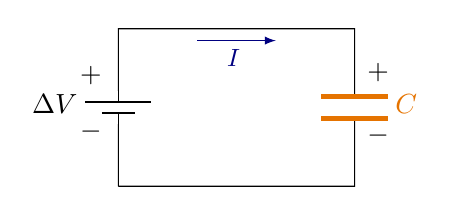
\begin{tikzpicture}
  \draw (0,0) to[mybattery] (0,2) -- (3,2)
              to[thick C] (3,0) -- (0,0);
  \node at (-0.35,0.7) {$-$};
  \node at (-0.35,1.4) {$+$};
  \node at (3.3,0.65) {$-$};
  \node at (3.3,1.45) {$+$};
  \draw[->,Icol] (1.0,1.85) --++ (1,0)
                 node[midway,left=1,below,scale=0.9] {$I$};
\end{tikzpicture}


% POLARIZED CAPACITOR with battery
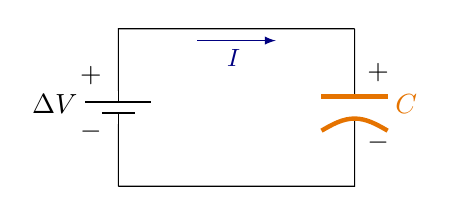
\begin{tikzpicture}
  \draw (0,0) to[mybattery] (0,2) -- (3,2)
        (0,0) -- (3,0) to[polar capacitor,color=Ccol,thick,Ccol,l_=$C$] (3,2);
              %to[polar capacitor,color=Ccol,thick,l=$C$,reverse] (3,0) -- (0,0);
  \node at (-0.35,0.7) {$-$};
  \node at (-0.35,1.4) {$+$};
  \node at (3.3,0.55) {$-$};
  \node at (3.3,1.45) {$+$};
  %\node at (3.7,0.95) {$C$};
  \draw[->,Icol] (1.0,1.85) --++ (1,0)
                 node[midway,left=1,below,scale=0.9] {$I$};
\end{tikzpicture}


% POLARIZED CAPACITOR with battery
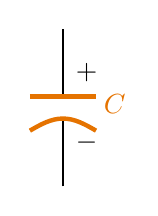
\begin{tikzpicture}
  \draw (0,0) to[polar capacitor,color=Ccol,thick,Ccol,l_=$C$] (0,2);
  \node at (0.3,0.55) {$-$};
  \node at (0.3,1.45) {$+$};
\end{tikzpicture}


% CAPACITORS in series
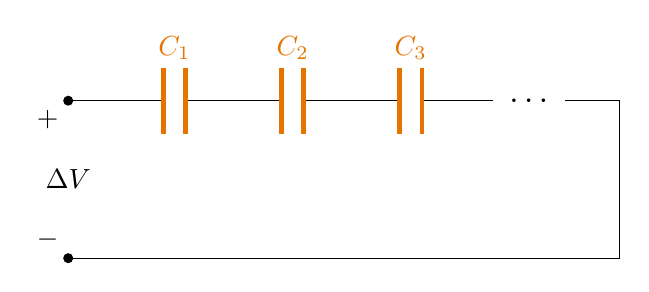
\begin{tikzpicture}
  \draw (0,2) to [short,*-] (0.6,2)
              to[thick C,l=$C_1$] ++(1.5,0)
              to[thick C,l=$C_2$] ++(1.5,0)
              to[thick C,l=$C_3$] ++(1.5,0)
              %(6,2) to[C,color=Ccol,thick,l=$C_4$]
              -- ++(1.5,0) node[midway,fill=white,inner sep=5,scale=1.2] {$.\,.\,.$}
              -- (7,2) -- (7,0) to[short,-*] (0,0);
  \node at (0,1) {$\Delta V$};
  \node[below left] at (0,2) {$+$};
  \node[above left] at (0,0) {$-$};
\end{tikzpicture}


% CAPACITORS in parallel
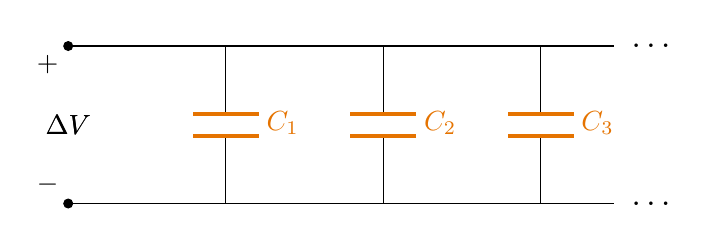
\begin{tikzpicture}
  \node[fill=white,inner sep=5,scale=1.2] (ET) at (7.4,2) {$.\,.\,.$};
  \node[fill=white,inner sep=5,scale=1.2] (EB) at (7.4,0) {$.\,.\,.$};
  \node at (0,1) {$\Delta V$};
  %\draw (0,0) to[battery1] (0,2) -- (2,2) to[C,color=Ccol,thick,l=$C_1$] (2,0) -- (0,0);
  \draw (0,2) to[short,*-] (2,2) to[thick C,l=$C_1$] (2,0) to[short,-*] (0,0);
  \draw (2,2) -- (4,2) to[thick C,l=$C_2$] (4,0) -- (2,0);
  \draw (4,2) -- (6,2) to[thick C,l=$C_3$] (6,0) -- (4,0);
  \draw (6,2) -- (ET.180);
  \draw (6,0) -- (EB.180);
  %\draw (6,2) -- (8,2) to[C,color=Ccol,thick,l=$C_4$] (8,0) -- (6,0);
  \node at (0,1) {$\Delta V$};
  \node[below left] at (0,2) {$+$};
  \node[above left] at (0,0) {$-$};
\end{tikzpicture}


\end{document}
